\documentclass[aspectratio=1610]{beamer}


\usepackage{listings}

\usepackage{xcolor}
\definecolor{pgreen}{rgb}{0,0.5,0}

\usetheme{Antibes}

\lstset{
    language=Java,
    showstringspaces=false,
    columns=flexible,
    basicstyle={\small\ttfamily},
    numbers=none,
    numberstyle=\tiny\color{gray},
    keywordstyle=\color{blue},
    commentstyle=\color{pgreen},
    stringstyle=\color{pgreen},
    breaklines=true,
    breakatwhitespace=true,
    tabsize=3,
    escapeinside={(*}{*)},
    aboveskip=-1em,
    belowskip=-1em,
}

%Information to be included in the title page:
\title{Incremental clone detection for IDEs using dynamic suffix arrays}
\author{Jakob Konrad Hansen}
\institute{University of Oslo}
\date{2023}



\begin{document}

\frame{\titlepage}

\begin{frame}
    \frametitle{Outline}
    \tableofcontents
\end{frame}

\section{Motivation and contribution}

\begin{frame}
\frametitle{Motivation}
\begin{itemize}
    \item Duplicated code is generally considered harmful to software quality
    \item Code clone detection, analysis and management is therefore important
    \item Incremental clone detection algorithms have not been thoroughly researched
    \item Incremental algorithms are useful in use-cases such as in IDEs
\end{itemize}
\end{frame}

\begin{frame}
\frametitle{Our contribution}
\begin{itemize}
    \item CCDetect-LSP: An incremental clone detection tool for IDEs
    \item Uses a novel application of dynamic extended suffix arrays for clone detection
    \item Language- and IDE agnostic via Tree-sitter and LSP
\end{itemize}
\end{frame}

\section{Background}

\subsection{Code clone theory}

\begin{frame}
    \frametitle{Code clones}

    \begin{definition}[Code snippet]
        A code snippet is a piece of contiguous source code in a larger software system.
    \end{definition}

    \begin{definition}[Code clone]
        A code clone is a code snippet which is equal or similar to another code snippet. The two
        code snippets are both code clones, and together they form a clone pair.
        Similarity is determined by some metric such as number of equal lines of code.
    \end{definition}
\end{frame}

\begin{frame}
	\frametitle{Clone types}
	\begin{itemize}
		\item Code clones are classified into four types
		      \begin{itemize}
			      \item Type-1: Syntactically identical
			      \item Type-2: Structurally identical
			      \item Type-3: Structurally similar
			      \item Type-4: Functionally similar (generally)
		      \end{itemize}
	\end{itemize}
\end{frame}


\begin{frame}[fragile]
	\frametitle{Clone type examples: type-1 and type-2}
    \begin{figure}[t]
		\begin{center}
			\begin{tabular}{c | c}
				\begin{lstlisting}
for (int i = 0; i < 10;   i++) {
    print(i);
}
\end{lstlisting} &
				\begin{lstlisting}
for (int i = 0; i < 10; i++) {
    // A comment

    print(i);
}
            \end{lstlisting}
			\end{tabular}
		\end{center}
        \caption{Type-1 clone pair}
    \end{figure}
    \begin{figure}[t]
        	\begin{center}
        \begin{tabular}{p{6cm} | p{6cm}}
\begin{lstlisting}
for (int i = 0; i < 10; i++) {
    print(i);
}
\end{lstlisting} & \begin{lstlisting}
for (int (*\textbf j*) = (*\textbf 5*); (*\textbf j*) < (*\textbf{20}*); (*\textbf j++*)) {
    print((*\textbf j*));
}
\end{lstlisting}
		\end{tabular}
	\end{center}

        \caption{Type-2 clone pair}
    \end{figure}

\end{frame}


\begin{frame}[fragile]
	\frametitle{Clone type examples: type-3 and type-4}
    \vspace{0.5cm}
	\begin{figure}[t]
		\begin{center}
			\begin{tabular}{p{6cm} | p{6cm}}
				\begin{lstlisting}
for (int i = 0; i < 10; i++) {
    print(i);
}\end{lstlisting} &
				\begin{lstlisting}
for (int i = 0; i < 10; i++) {
    print(i);
    print(i*2);
}\end{lstlisting}
			\end{tabular}
		\end{center}
		\caption{Type-3 clone pair}
		\label{fig:type3clone}
	\end{figure}
    \vspace{-0.5cm}

	\begin{figure}[t]
		\begin{center}
			\begin{tabular}{r | p{6.5cm}}
				\hspace{3.2cm}\begin{lstlisting}
print((n*(n-1))/2)
\end{lstlisting} &
				\begin{lstlisting}
int sum = 0;
for (int i = 0; i < n; i++) {
    for (int j = i+1; j < n; j++) {
        sum++;
    }
}
print(sum);
            \end{lstlisting}
			\end{tabular}
		\end{center}
		\caption{Type-4 clone pair}
		\label{fig:type4clone}
	\end{figure}
\end{frame}

\begin{frame}{Clone detection}
    \begin{figure}
        \begin{center}
            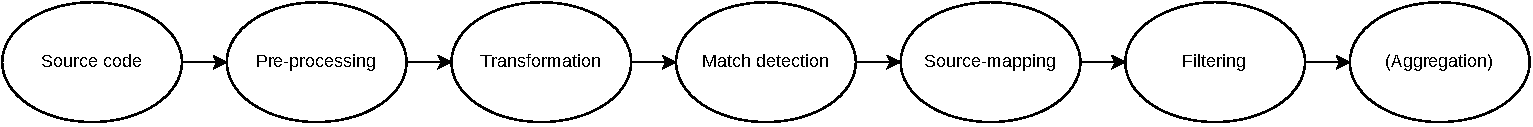
\includegraphics[width=0.95\textwidth]{figures/detectionphases.drawio.pdf}
        \end{center}
    \end{figure}
\end{frame}

\begin{frame}{Clone matching techniques}
    \begin{itemize}
        \item Text-based detection
            \begin{itemize}
                \item Match based on raw source code
            \end{itemize}
        \item Token-based detection
            \begin{itemize}
                \item Match based on tokens
            \end{itemize}
        \item Syntactic detection
            \begin{itemize}
                \item Match based on AST
            \end{itemize}
        \item Hybrid detection
            \begin{itemize}
                \item Combine multiple approaches
            \end{itemize}
    \end{itemize}
\end{frame}


\subsection{Preliminary algorithms and data structures}
\begin{frame}{Suffix array}
\end{frame}

\section{Implementation}

\subsection{LSP architecture and functionality + demo}

\begin{frame}{Implementation: LSP architecture and functionality}
	\begin{itemize}
		\item The Language Server Protocol (LSP) facilitates IDE agnostic tooling
		\item CCDetect-LSP is implemented as an LSP server
	\end{itemize}
\end{frame}

\subsection{Initial clone detection}

\begin{frame}{Implementation: Initial clone detection}
\end{frame}

\subsection{Incremental clone detection}
\begin{frame}{Implementation: Incremental clone detection}
\end{frame}

\section{Evaluation}
\begin{frame}{Results}
\end{frame}

\section{Discussion}
\begin{frame}{Discussion}
\end{frame}

\section{Conclusion}
\begin{frame}{Conclusion}
\end{frame}

\end{document}
